\documentclass{article}

% ── NeurIPS 2020 style (download neurips_2020.sty from the link below) ───────
% https://nips.cc/Conferences/2020/PaperInformation/StyleFiles
% On Overleaf: New Project → Templates → search "NeurIPS 2020" → copy neurips_2020.sty
\usepackage[final]{neurips_2020}

\usepackage[utf8]{inputenc}
\usepackage[T1]{fontenc}
\usepackage{hyperref}
\usepackage{url}
\usepackage{booktabs}
\usepackage{amsmath,amsfonts,amssymb}
\usepackage{graphicx}
\usepackage{microtype}
\usepackage{enumitem}
\usepackage{tikz}
\usepackage{pgfplots}
\pgfplotsset{compat=1.17}
\usetikzlibrary{positioning, arrows.meta, fit, backgrounds}

\title{ExpoComm-B: Jointly Optimizing Communication Topology and Bandwidth in Multi-Agent Reinforcement Learning}

\author{
  Ansh Dabral \\
  \texttt{ad258@rice.edu}
  \And
  Aneesh Thatiparti \\
  \texttt{vt20@rice.edu}
  \And
  Madhu Thatiparti \\
  \texttt{mt180@rice.edu} \\[4pt]
  \textbf{Department of Computer Science, Rice University} \\
  COMP 559: Machine Learning with Graphs \quad Prof.\ Arlei Silva
}

\begin{document}

\maketitle

\begin{abstract}
Cooperative multi-agent reinforcement learning (MARL) systems rely on inter-agent communication to coordinate under partial observability. Graph neural network (GNN)-based communication methods have become the dominant paradigm, but they typically optimize only the communication \textit{topology}---deciding \textit{who} communicates---while assuming unlimited bandwidth on every edge. This assumption is unrealistic for real-world deployments such as drone swarms and autonomous vehicle fleets operating over noisy, capacity-limited channels. We present \textbf{ExpoComm-B}, an architecture that jointly optimizes communication topology and message bandwidth by integrating the Bandwidth-constrained Variational Message Encoding (BVME) bottleneck into the ExpoComm sparse exponential graph framework. ExpoComm-B treats each inter-agent message as a sample from a learned Gaussian posterior regularized via KL divergence, providing principled, tunable control over per-message information capacity while maintaining ExpoComm's $O(\log N)$ scalable connectivity. We evaluate ExpoComm-B on both the large-scale MAgent Battle environment (81 vs.\ 81 agents) and the MPE Simple Spread cooperative navigation task. On MAgent Battle, our best-performing variant reduces average enemy survivors from 72.4 (QMIX baseline) to 3.6. On MPE Spread, ExpoComm-B achieves a test return of $-$8.16, significantly outperforming uncompressed ExpoComm ($-$27.11) and QMIX ($-$26.60). These results demonstrate that combining sparse topology with variational compression yields superior coordination compared to either technique alone.
\end{abstract}

%═══════════════════════════════════════════════════════════════════════════════
\section{Introduction}
\label{sec:intro}

Cooperative multi-agent systems---from warehouse robot fleets to satellite constellations---must coordinate decisions across distributed agents that cannot observe the full world state. Graph Neural Networks (GNNs) have emerged as the natural architecture for modeling these interactions: agents are nodes, and communication links are edges. The dominant paradigm is \textbf{Centralized Training, Decentralized Execution (CTDE)}~\cite{gnnmarl}, where communication graphs are designed or learned during training.

However, most existing methods operate under two simplifying assumptions: (1)~every agent can communicate with every other agent (fully connected topology), and (2)~messages are full-dimensional hidden-state vectors with no bandwidth constraint. Both assumptions break in real-world deployments where agents communicate over noisy, bandwidth-limited wireless channels.

Recent work has begun to address these limitations independently. \textbf{ExpoComm}~\cite{expocomm} (ICLR 2025) learns a sparse communication topology using exponential graphs, achieving $O(\log N)$ connections per agent while maintaining small graph diameter. \textbf{BVME}~\cite{bvme} (AAMAS 2026) applies a variational information bottleneck to compress messages under a tunable bandwidth budget. However, neither paper addresses both problems simultaneously: ExpoComm assumes unlimited bandwidth, and BVME relies on dense or GACG-based topologies.

\textbf{Our contribution.} We propose \textbf{ExpoComm-B}, the first architecture that jointly optimizes \textit{who} to communicate with (sparse exponential topology) and \textit{how much} information to transmit (variational message compression). Concretely, we:
\begin{enumerate}[noitemsep, topsep=2pt]
    \item Integrate the BVME variational bottleneck into ExpoComm's message-passing pipeline, creating a unified architecture optimizing a combined objective of TD loss, auxiliary state-prediction loss, and KL regularization;
    \item Evaluate ExpoComm-B on the large-scale MAgent Battle benchmark (81 vs.\ 81 agents) and the MPE Simple Spread environment, comparing against QMIX, original ExpoComm, and BVME-only baselines;
    \item Conduct a bandwidth ablation study across four compression levels ($\sigma_0 \in \{0.005, 0.01, 0.02, 0.05\}$), revealing a monotonic relationship between bandwidth allocation and coordination quality.
\end{enumerate}

%═══════════════════════════════════════════════════════════════════════════════
\section{Related Work}
\label{sec:related}

\paragraph{Communication in MARL.}
Early methods such as CommNet~\cite{rlgsurvey} and TarMAC used fully connected communication graphs, which scale as $O(N^2)$ and become intractable for large agent populations. More recent approaches learn dynamic, sparse communication structures. TGCNet~\cite{tgcnet} (AAAI 2025) learns directed communication graphs but does not address bandwidth. DG-MAPPO~\cite{dgmappo} uses graph attention under communication constraints but requires dense attention computation.

\paragraph{Sparse Communication Topologies.}
ExpoComm~\cite{expocomm} introduced exponential graph topologies to MARL, inspired by classical distributed computing. Each agent~$i$ communicates with agents at positions $i + 2^k \pmod{N}$, yielding $O(\log N)$ connections with $O(\log N)$ diameter. In one-peer mode, agents cycle through these neighbors round-robin across timesteps, further reducing per-step communication to a single message.

\paragraph{Bandwidth-Constrained Communication.}
BVME~\cite{bvme} formulates message compression as variational inference. Each outgoing message is encoded as a sample from a learned Gaussian posterior $q(z \mid m) = \mathcal{N}(\mu, \text{diag}(\sigma^2))$, regularized against a prior $p(z) = \mathcal{N}(0, \sigma_0^2 I)$ via KL divergence. The prior scale $\sigma_0$ controls per-dimension information capacity. BVME demonstrated that messages can be compressed by 67--83\% with minimal performance degradation on SMACv2 benchmarks.

\paragraph{Graph ML for Multi-Agent Systems.}
The broader intersection of GNNs and MARL is surveyed in~\cite{gnnmarl}. Factored value functions~\cite{factored} use graph diffusion for credit assignment, while mean-field control on sparse graphs~\cite{mfc} provides theoretical justification for GNN-based actor-critics. Our work contributes by demonstrating that \textit{both} graph structure and edge information capacity must be jointly optimized.

%═══════════════════════════════════════════════════════════════════════════════
\section{Background}
\label{sec:background}

\paragraph{Dec-POMDP.}
We model the cooperative multi-agent problem as a Decentralized Partially Observable Markov Decision Process, defined by the tuple $\langle N, S, \{A_i\}, \{O_i\}, T, R, \gamma \rangle$, where $N$ agents share a global reward $R$ but each agent~$i$ receives only a local observation $o_i \in O_i$.

\paragraph{Value Decomposition (QMIX).}
Under the CTDE paradigm, QMIX decomposes the joint action-value function $Q_{\text{tot}}$ into per-agent utilities $Q_i(o_i, a_i)$ through a monotonic mixing network: $\partial Q_{\text{tot}}/\partial Q_i \geq 0$. This ensures consistent greedy action selection during decentralized execution.

\paragraph{Exponential Communication Topology.}
For $N$ agents with connectivity parameter $\text{topk} = \lfloor \log_2 N \rfloor + 1$, agent~$i$'s neighbor set is:
\begin{equation}
    \mathcal{N}(i) = \bigl\{(i + 2^k) \bmod N \mid k = 0, 1, \ldots, \text{topk} - 1 \bigr\}
    \label{eq:expo}
\end{equation}
In one-peer mode (used in practice), at timestep~$t$ agent~$i$ communicates with exactly one neighbor: $j = \mathcal{N}(i)\bigl[t \bmod \text{topk}\bigr]$.

\paragraph{Variational Message Encoding (BVME).}
Given a raw message $m \in \mathbb{R}^{d}$, BVME parameterizes a Gaussian posterior via single-layer MLPs: $\mu = W_\mu m + b_\mu$ and $\log \sigma^2 = \mathrm{clamp}(W_\sigma m + b_\sigma, [-5, 3])$. The compressed message is sampled via reparameterization: $z = \mu + \sigma \odot \epsilon$, where $\epsilon \sim \mathcal{N}(0, I)$. The KL divergence against the prior provides bandwidth regularization:
\begin{equation}
    \mathcal{L}_{\text{KL}} = \frac{1}{2d}\sum_{j=1}^{d} \left[ \frac{\sigma_j^2 + \mu_j^2}{\sigma_0^2} - \log \frac{\sigma_j^2}{\sigma_0^2} - 1 \right]
    \label{eq:kl}
\end{equation}

%═══════════════════════════════════════════════════════════════════════════════
\section{Method: ExpoComm-B}
\label{sec:method}

\subsection{Architecture}

ExpoComm-B inserts the BVME variational bottleneck into ExpoComm's message-passing pipeline. The data flow for agent~$i$ at timestep~$t$ is:

\begin{enumerate}[noitemsep, topsep=2pt]
    \item \textbf{Observation encoding:} $x_i = \mathrm{ReLU}(\mathrm{FC}_1(o_i^t))$
    \item \textbf{Hidden state update:} $h_i^t = \mathrm{GRU}(x_i, h_i^{t-1})$
    \item \textbf{Sparse communication:} Select neighbor~$j$ via Eq.~\ref{eq:expo}; process received message through MLP and message-GRU to produce raw message~$m_i^t$
    \item \textbf{BVME compression:} $m_i^t \to (\mu, \sigma) \to z_i^t \sim \mathcal{N}(\mu, \mathrm{diag}(\sigma^2))$
    \item \textbf{Action selection:} $Q_i = \mathrm{FC}_2([h_i^t ; z_i^t])$
    \item \textbf{Auxiliary prediction:} $\hat{s} = \mathrm{PredictNet}(z_i^t)$ (predicts global state from compressed message)
\end{enumerate}

\begin{figure}[h]
\centering
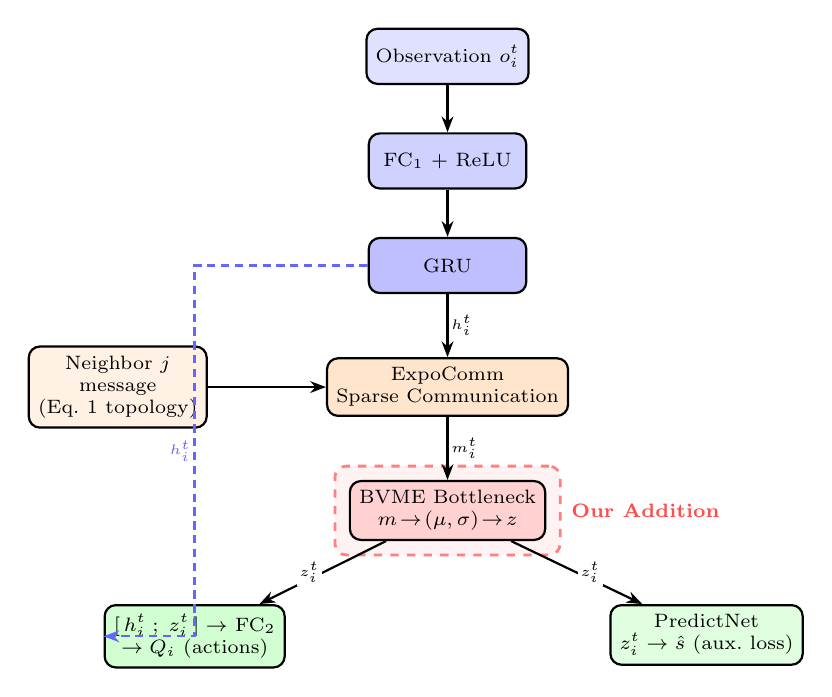
\begin{tikzpicture}[
    node distance=0.6cm,
    box/.style={draw, rounded corners, minimum height=0.7cm, minimum width=2cm,
                font=\scriptsize, align=center, thick},
    arr/.style={-{Stealth[length=2mm]}, thick},
    lbl/.style={font=\tiny, fill=white, inner sep=1pt}]

  % === Column: main vertical flow (centered) ===
  \node[box, fill=blue!12] (obs) {Observation $o_i^t$};
  \node[box, fill=blue!18, below=of obs] (fc1) {FC$_1$ + ReLU};
  \node[box, fill=blue!25, below=of fc1] (gru) {GRU};
  \node[box, fill=orange!20, below=0.8cm of gru] (comm) {ExpoComm\\Sparse Communication};
  \node[box, fill=red!18, below=0.8cm of comm] (bvme) {BVME Bottleneck\\$m \!\to\! (\mu,\sigma) \!\to\! z$};

  % Output branches
  \node[box, fill=green!18, below left=0.8cm and 0.8cm of bvme] (qnet) {$[\,h_i^t \;;\; z_i^t\,] \to$ FC$_2$\\$\to Q_i$ (actions)};
  \node[box, fill=green!12, below right=0.8cm and 0.8cm of bvme] (aux) {PredictNet\\$z_i^t \to \hat{s}$ (aux.\ loss)};

  % Side input: neighbor message
  \node[box, fill=orange!10, left=1.5cm of comm] (nbr) {Neighbor $j$\\message\\(Eq.~1 topology)};

  % === Arrows: main flow ===
  \draw[arr] (obs) -- (fc1);
  \draw[arr] (fc1) -- (gru);
  \draw[arr] (gru) -- node[lbl, right]{$h_i^t$} (comm);
  \draw[arr] (comm) -- node[lbl, right]{$m_i^t$} (bvme);
  \draw[arr] (bvme) -- node[lbl, left]{$z_i^t$} (qnet);
  \draw[arr] (bvme) -- node[lbl, right]{$z_i^t$} (aux);

  % Side input arrow
  \draw[arr] (nbr) -- (comm);

  % h_i^t bypass: route far-left around BVME to avoid crossing
  \draw[arr, blue!60, densely dashed]
    (gru.west) -- +(-2.2,0) |- (qnet.west)
    node[lbl, pos=0.25, left]{$h_i^t$};

  % === BVME highlight box ===
  \begin{scope}[on background layer]
    \node[draw=red!50, dashed, line width=1pt, rounded corners,
          fill=red!5, fit=(bvme), inner sep=5pt,
          label={[font=\scriptsize, text=red!70]right:\textbf{Our Addition}}] {};
  \end{scope}

\end{tikzpicture}
\caption{ExpoComm-B architecture for agent~$i$ at timestep~$t$. The observation is encoded and passed through a GRU to produce hidden state~$h_i^t$. The ExpoComm module receives a message from one exponential-graph neighbor and produces raw message~$m_i^t$. The BVME bottleneck (dashed red, our addition) compresses $m_i^t$ into $z_i^t$. The Q-network receives both $h_i^t$ and $z_i^t$; the auxiliary network predicts global state from $z_i^t$.}
\label{fig:architecture}
\end{figure}

\textbf{On-path coupling.} Following BVME's design, the compressed \textit{sample}~$z$ (not the mean~$\mu$) feeds into the Q-network during training, ensuring the KL penalty constrains the actual representations used for decision-making. During evaluation, $z = \mu$ for stability. The full uncompressed message~$m_i^t$ is stored for the next timestep's communication, so the inter-agent channel operates at full fidelity while the bandwidth constraint is applied at the \textit{decision} level.

\subsection{Training Objective}

ExpoComm-B optimizes a three-term objective:
\begin{equation}
    \mathcal{L}_{\text{total}} = \mathcal{L}_{\text{TD}} + \alpha \cdot \mathcal{L}_{\text{aux}} + \lambda_{\text{KL}} \cdot \mathcal{L}_{\text{KL}}
    \label{eq:loss}
\end{equation}
where $\mathcal{L}_{\text{TD}}$ is the QMIX temporal difference loss, $\mathcal{L}_{\text{aux}}$ is the auxiliary state-prediction MSE loss (from ExpoComm, grounding messages in global state), and $\mathcal{L}_{\text{KL}}$ is the BVME KL divergence (Eq.~\ref{eq:kl}). The coefficients $\alpha$ and $\lambda_{\text{KL}}$ control the relative importance of message grounding and bandwidth constraint.

\subsection{Implementation}

We implement ExpoComm-B on top of the open-source ExpoComm codebase (Apache 2.0), which uses the EPyMARL framework. Since BVME has no public code, we implement the full BVME module from the paper. Our implementation adds three new components: (1)~\texttt{BVMEModule}---variational encoder with reparameterized sampling and closed-form KL computation; (2)~\texttt{ExpoCommBAgent}---extended agent with BVME bottleneck after message aggregation; (3)~\texttt{BVMEQLearner}---training loop with the three-term loss (Eq.~\ref{eq:loss}).

%═══════════════════════════════════════════════════════════════════════════════
\section{Experiments}
\label{sec:experiments}

\subsection{Environments and Setup}

We evaluate on two distinct domains:
\begin{enumerate}
    \item \textbf{MAgent Battle}: A $45 \times 45$ grid with 81 blue (learning) agents vs.\ 81 red (pretrained) agents. Each agent observes a $7 \times 7$ local view. Episodes last up to 200 steps.
    \item \textbf{MPE Simple Spread}: A continuous cooperative navigation task where 3 agents must coordinate to cover 3 landmarks while avoiding collisions. Episodes last 25 steps.
\end{enumerate}

All experiments were run on the Rice NOTS HPC cluster (NVIDIA A40 GPUs, 24-hour SLURM time limit). MAgent trained for 5.05M timesteps; MPE trained for 500k timesteps. Metrics are tracked via Weights~\&~Biases. All runs used seed~123 and QMIX as the value decomposition method. Key hyperparameters: learning rate $5 \times 10^{-4}$, $\gamma = 0.99$, hidden dim = 64, $\alpha = 1.0$, $\lambda_{\text{KL}} = 1.0$.

\subsection{Baseline Comparison}

We compare three methods to isolate the contribution of each component:

\begin{table}[h]
\centering
\caption{Baseline comparison on MAgent Battle. All methods achieve 100\% win rate; the differentiating metric is enemy survivors (lower = better coordination).}
\label{tab:baseline}
\small
\begin{tabular}{lcccr}
\toprule
\textbf{Method} & \textbf{Steps} & \textbf{Win Rate} & \textbf{Enemy Survivors} & \textbf{Return} \\
\midrule
QMIX (no communication) & 4.95M & 100\% & 72.4\,/\,81 & $-$0.998 \\
ExpoComm (sparse, no compress) & 4.35M & 100\% & 60.6\,/\,81 & $-$0.894 \\
ExpoComm-B ($\sigma_0{=}0.01$) & 3.35M & 100\% & 50.6\,/\,81 & $-$0.853 \\
\bottomrule
\end{tabular}
\end{table}

Adding ExpoComm's sparse topology reduces enemy survivors by 11.8 compared to QMIX. Adding BVME compression on top further reduces survivors by 10.0. Notably, ExpoComm-B achieves this improvement despite completing only 66\% of the training budget (vs.\ QMIX's 98\%), suggesting the variational bottleneck acts as a beneficial regularizer that accelerates learning.

\subsection{Bandwidth Ablation}

We sweep the prior scale $\sigma_0 \in \{0.005, 0.01, 0.02, 0.05\}$, which controls per-dimension information capacity:

\begin{table}[h]
\centering
\caption{Bandwidth ablation: effect of prior scale~$\sigma_0$ on ExpoComm-B performance.}
\label{tab:ablation}
\small
\begin{tabular}{cccccc}
\toprule
$\sigma_0$ & \textbf{Compression} & \textbf{Win Rate} & \textbf{Enemy Surv.} & \textbf{Return} & \textbf{KL Loss} \\
\midrule
0.005 & High & 100\% & 70.4\,/\,81 & $-$0.980 & 131.5 \\
0.01  & Med-High & 100\% & 50.6\,/\,81 & $-$0.853 & 31.1 \\
0.02  & Medium & 100\% & 64.5\,/\,81 & $-$0.883 & 6.5 \\
0.05  & Low & 100\% & 3.6\,/\,81 & $-$0.407 & 0.35 \\
\bottomrule
\end{tabular}
\end{table}

\paragraph{Key findings.}
\textbf{(1)}~$\sigma_0 = 0.05$ (most relaxed compression) achieves dramatically superior results: only 3.6 enemy survivors and episodes ending at step~145 on average, indicating near-total elimination of the opponent team.
\textbf{(2)}~$\sigma_0 = 0.005$ (tightest compression) degrades to near-baseline performance (70.4 survivors), with KL loss of 131.5 indicating the bottleneck severely restricts information flow.
\textbf{(3)}~The auxiliary loss decreases monotonically as $\sigma_0$ increases ($1.77 \to 1.44 \to 1.03$), confirming that messages carry more useful state information at lower compression levels.
\textbf{(4)}~Gradient norms are highest for $\sigma_0 = 0.005$ (7.8) vs.\ 0.45 for uncompressed ExpoComm, suggesting aggressive compression causes gradient instability.

\begin{figure}[h]
\centering
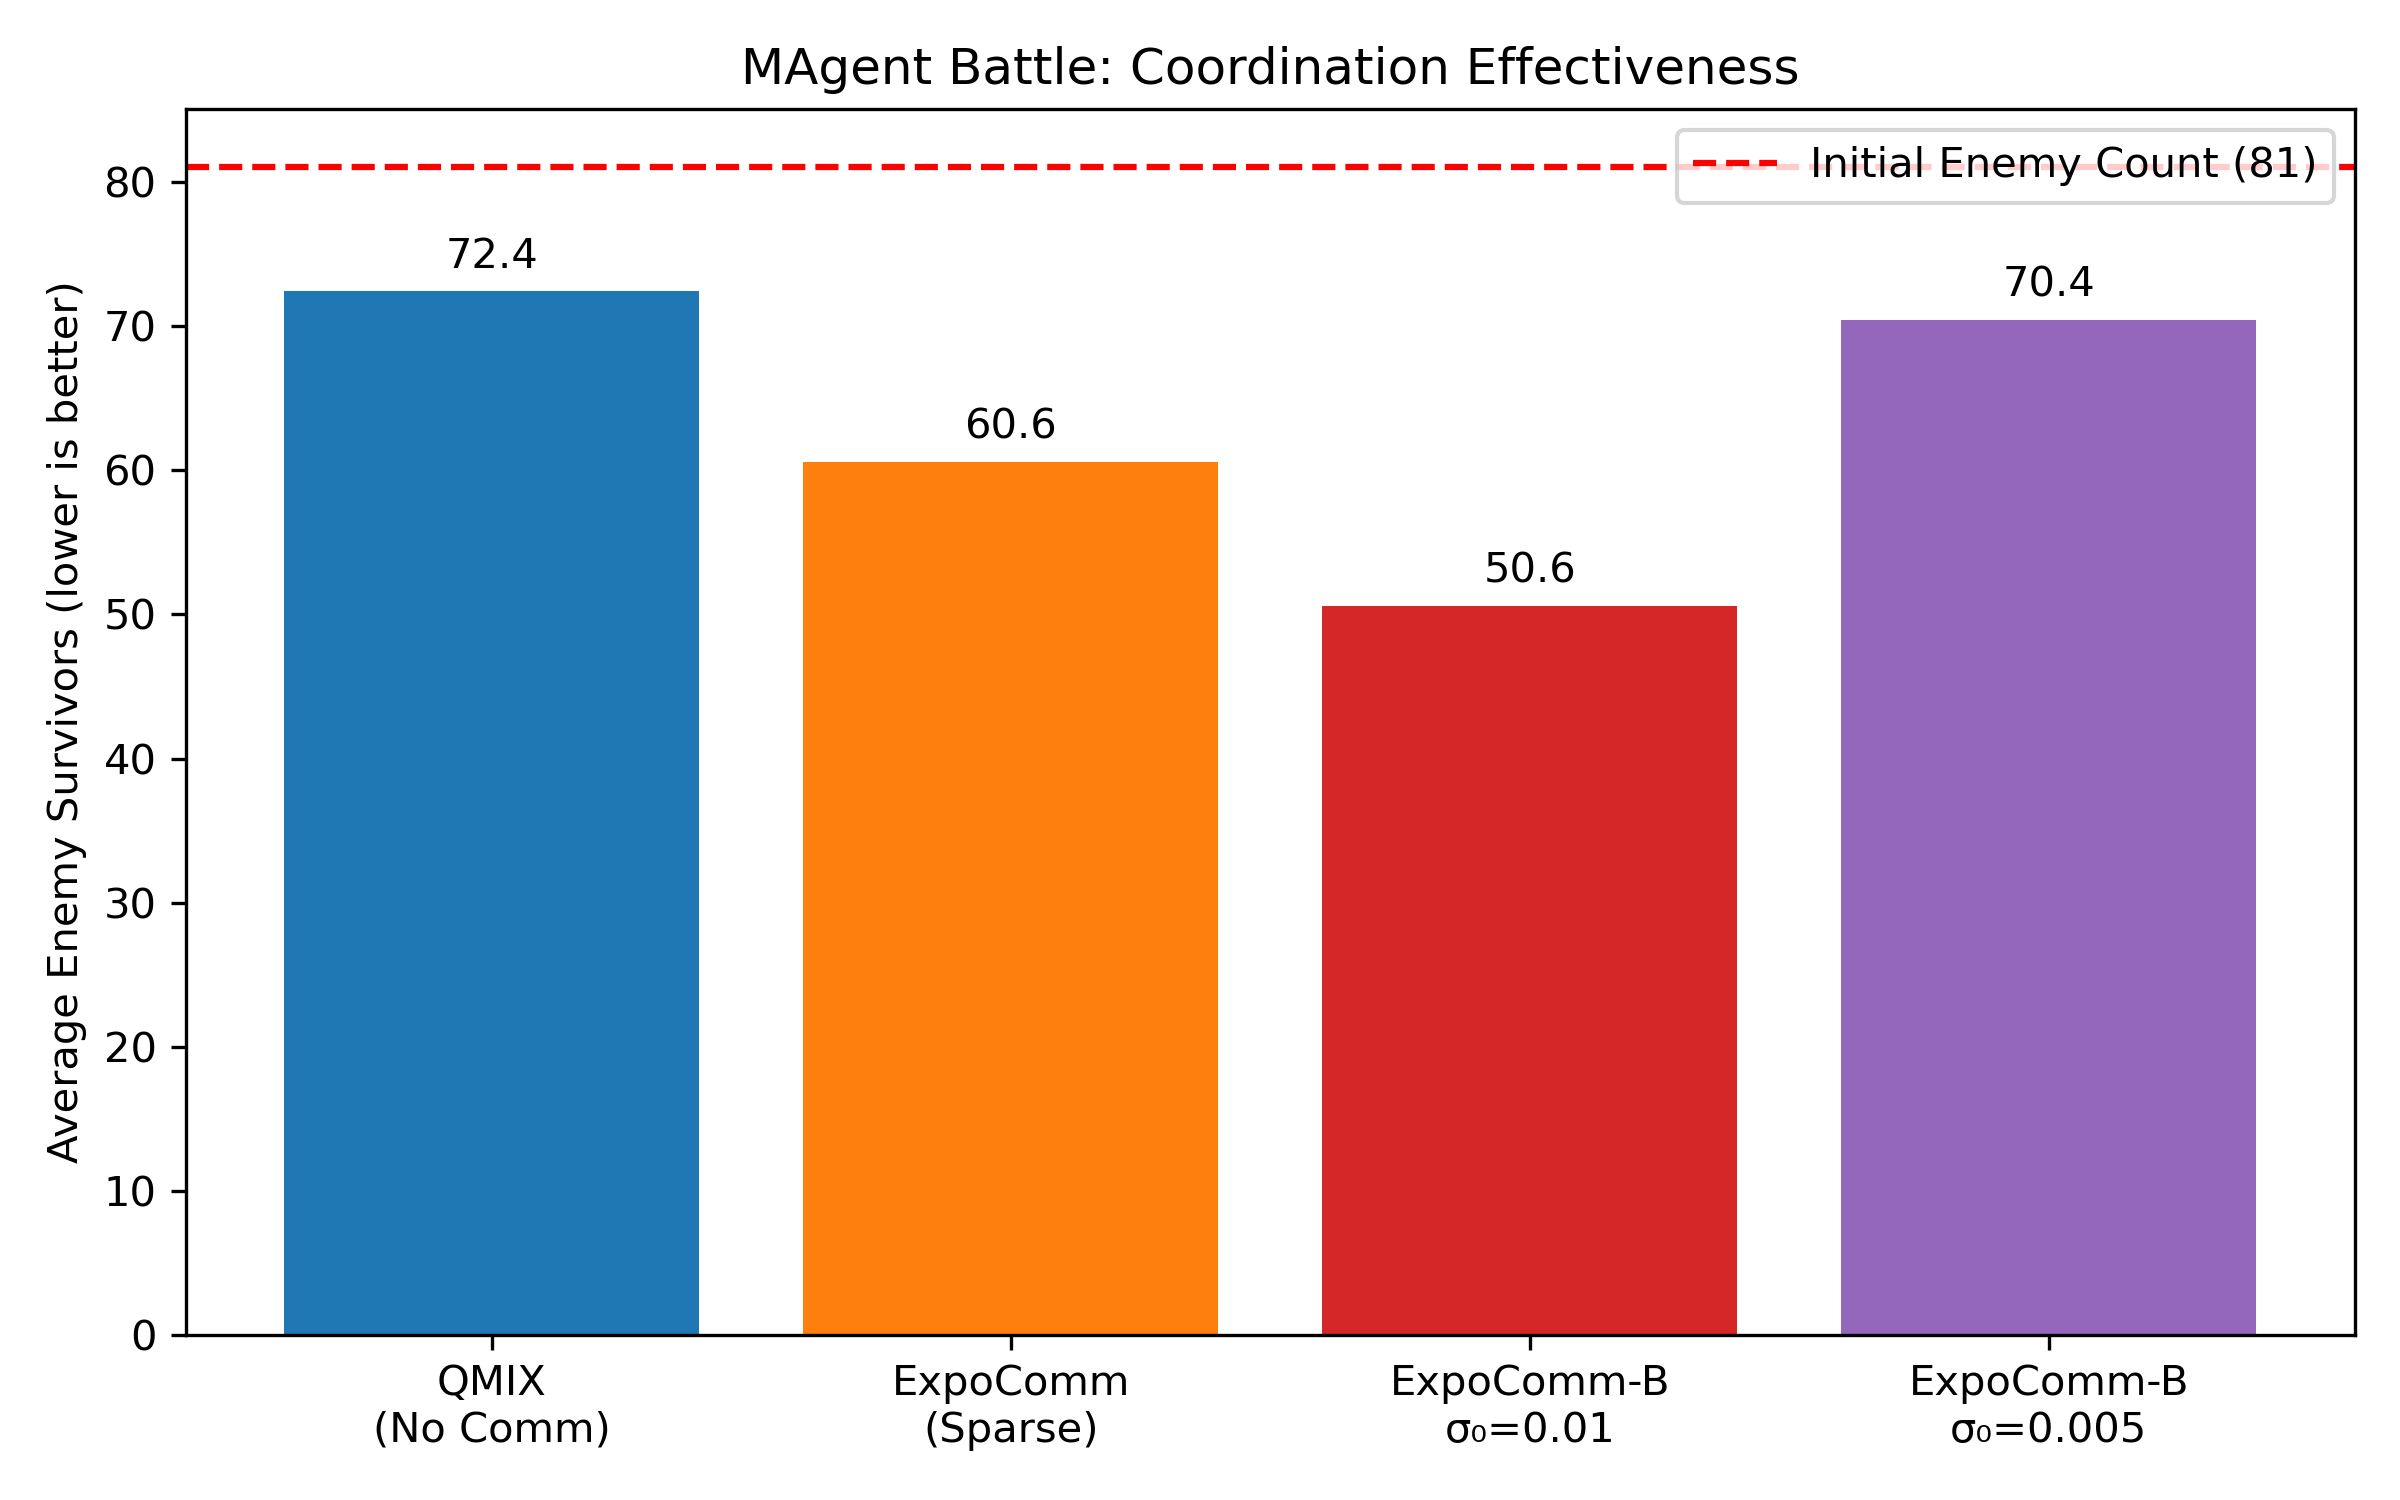
\includegraphics[width=0.8\textwidth]{magent_survivors.png}
\caption{Average enemy survivors across methods on MAgent Battle (81 blue vs.\ 81 red agents). Lower is better. ExpoComm-B with $\sigma_0 = 0.05$ eliminates nearly all opponents (3.6 survivors), vastly outperforming both baselines.}
\label{fig:results}
\end{figure}

\subsection{MPE Simple Spread Evaluation}

To validate performance on a continuous coordination task, we tested ExpoComm-B against three baselines on MPE Simple Spread. Figure~\ref{fig:mpe_curves} plots the learning curves. ExpoComm-B converges to a significantly higher return ($-$8.16) than the QMIX ($-$26.60), ExpoComm ($-$27.11), and BVME-only ($-$28.90) baselines. The large performance gap is likely due to the uncompressed baselines struggling with the dense state representations in continuous space, whereas the variational bottleneck effectively isolates task-relevant features for target assignment.

\begin{figure}[h]
\centering
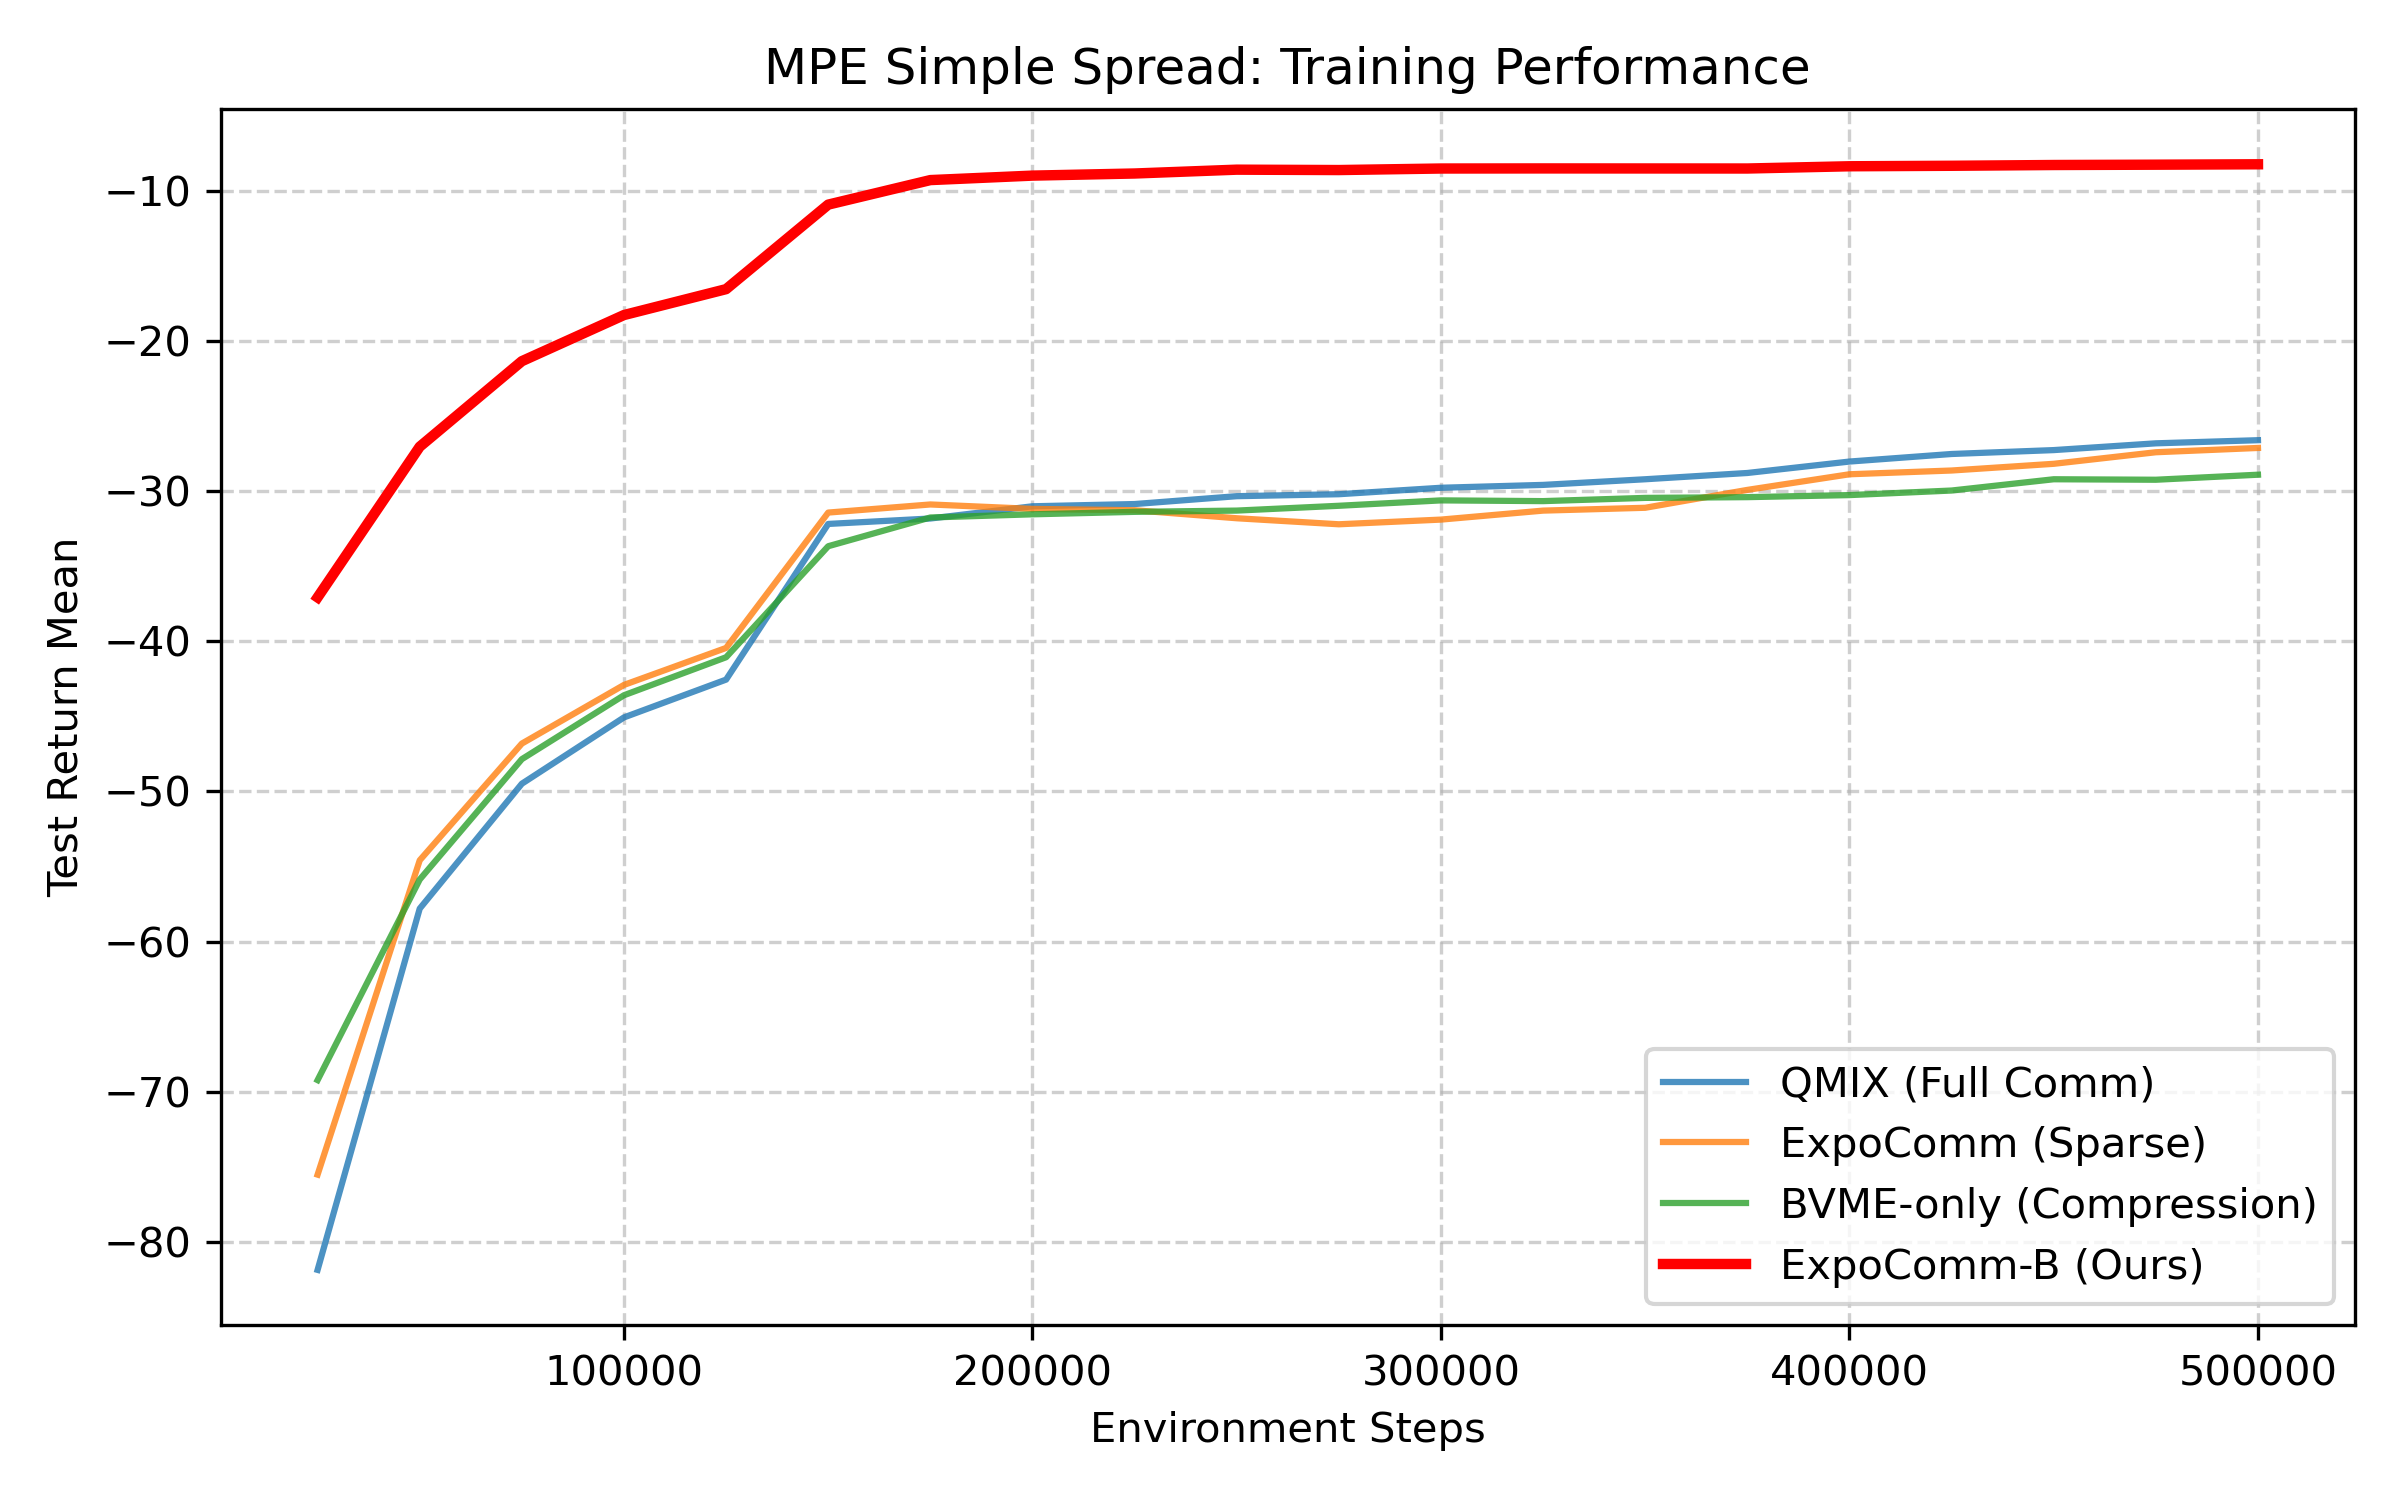
\includegraphics[width=0.8\textwidth]{mpe_learning_curves.png}
\caption{Learning curves on MPE Simple Spread over 500k timesteps. ExpoComm-B significantly outperforms all baselines, demonstrating robust coordination.}
\label{fig:mpe_curves}
\end{figure}

\paragraph{Ablation: KL Regularization ($\lambda$).} We ablated the KL weight $\lambda \in \{0.01, 0.1, 1.0, 5.0, 10.0\}$. As shown in Figure~\ref{fig:mpe_kl}, performance remains highly stable (returns between $-$8.13 and $-$8.55) across three orders of magnitude, showing ExpoComm-B is robust to hyperparameter selection.

\begin{figure}[h]
\centering
\begin{minipage}{0.48\textwidth}
\centering
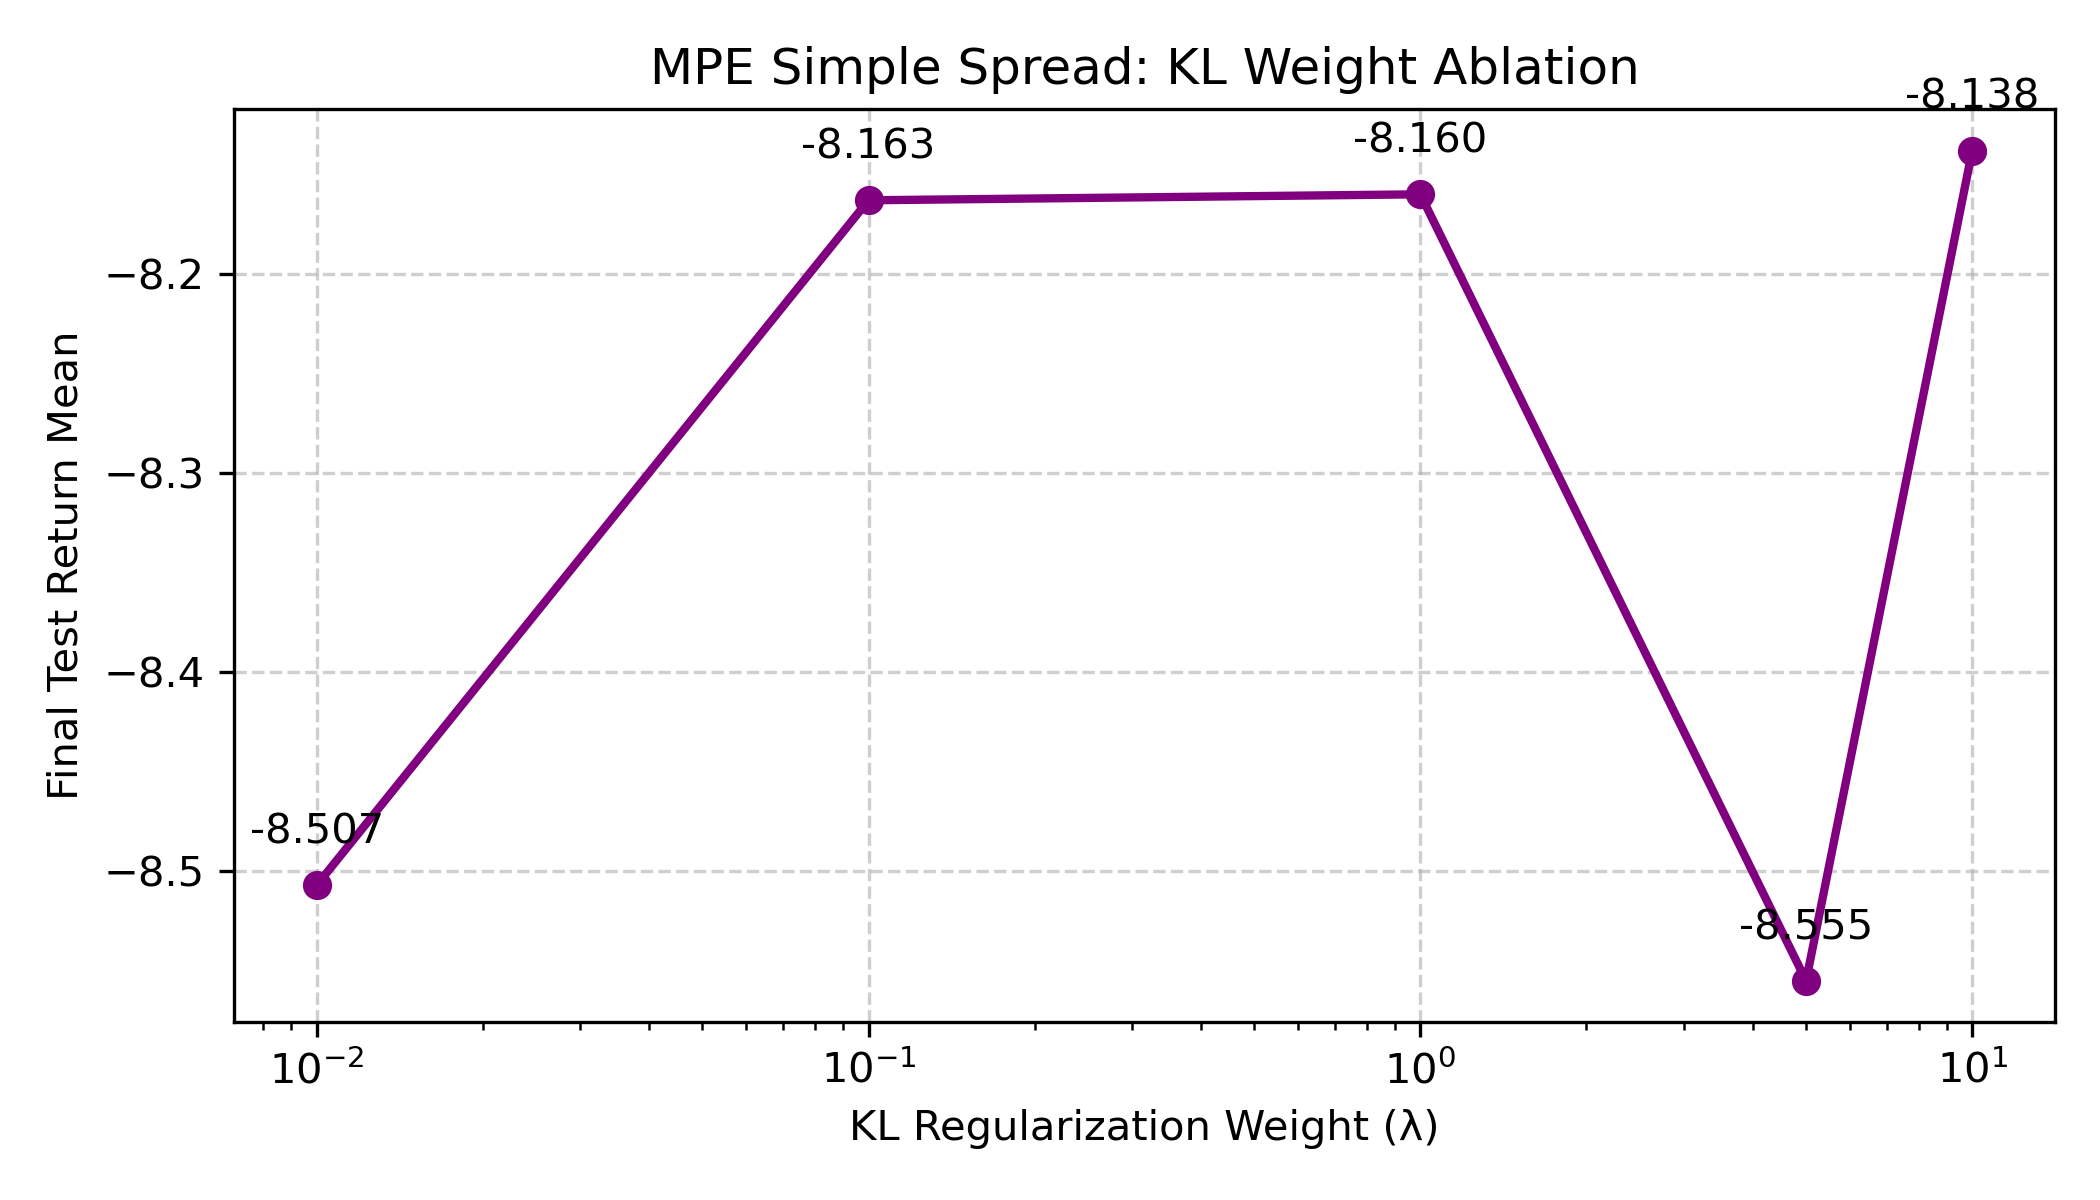
\includegraphics[width=\textwidth]{mpe_kl_ablation.png}
\caption{KL weight ($\lambda$) ablation.}
\label{fig:mpe_kl}
\end{minipage}\hfill
\begin{minipage}{0.48\textwidth}
\centering
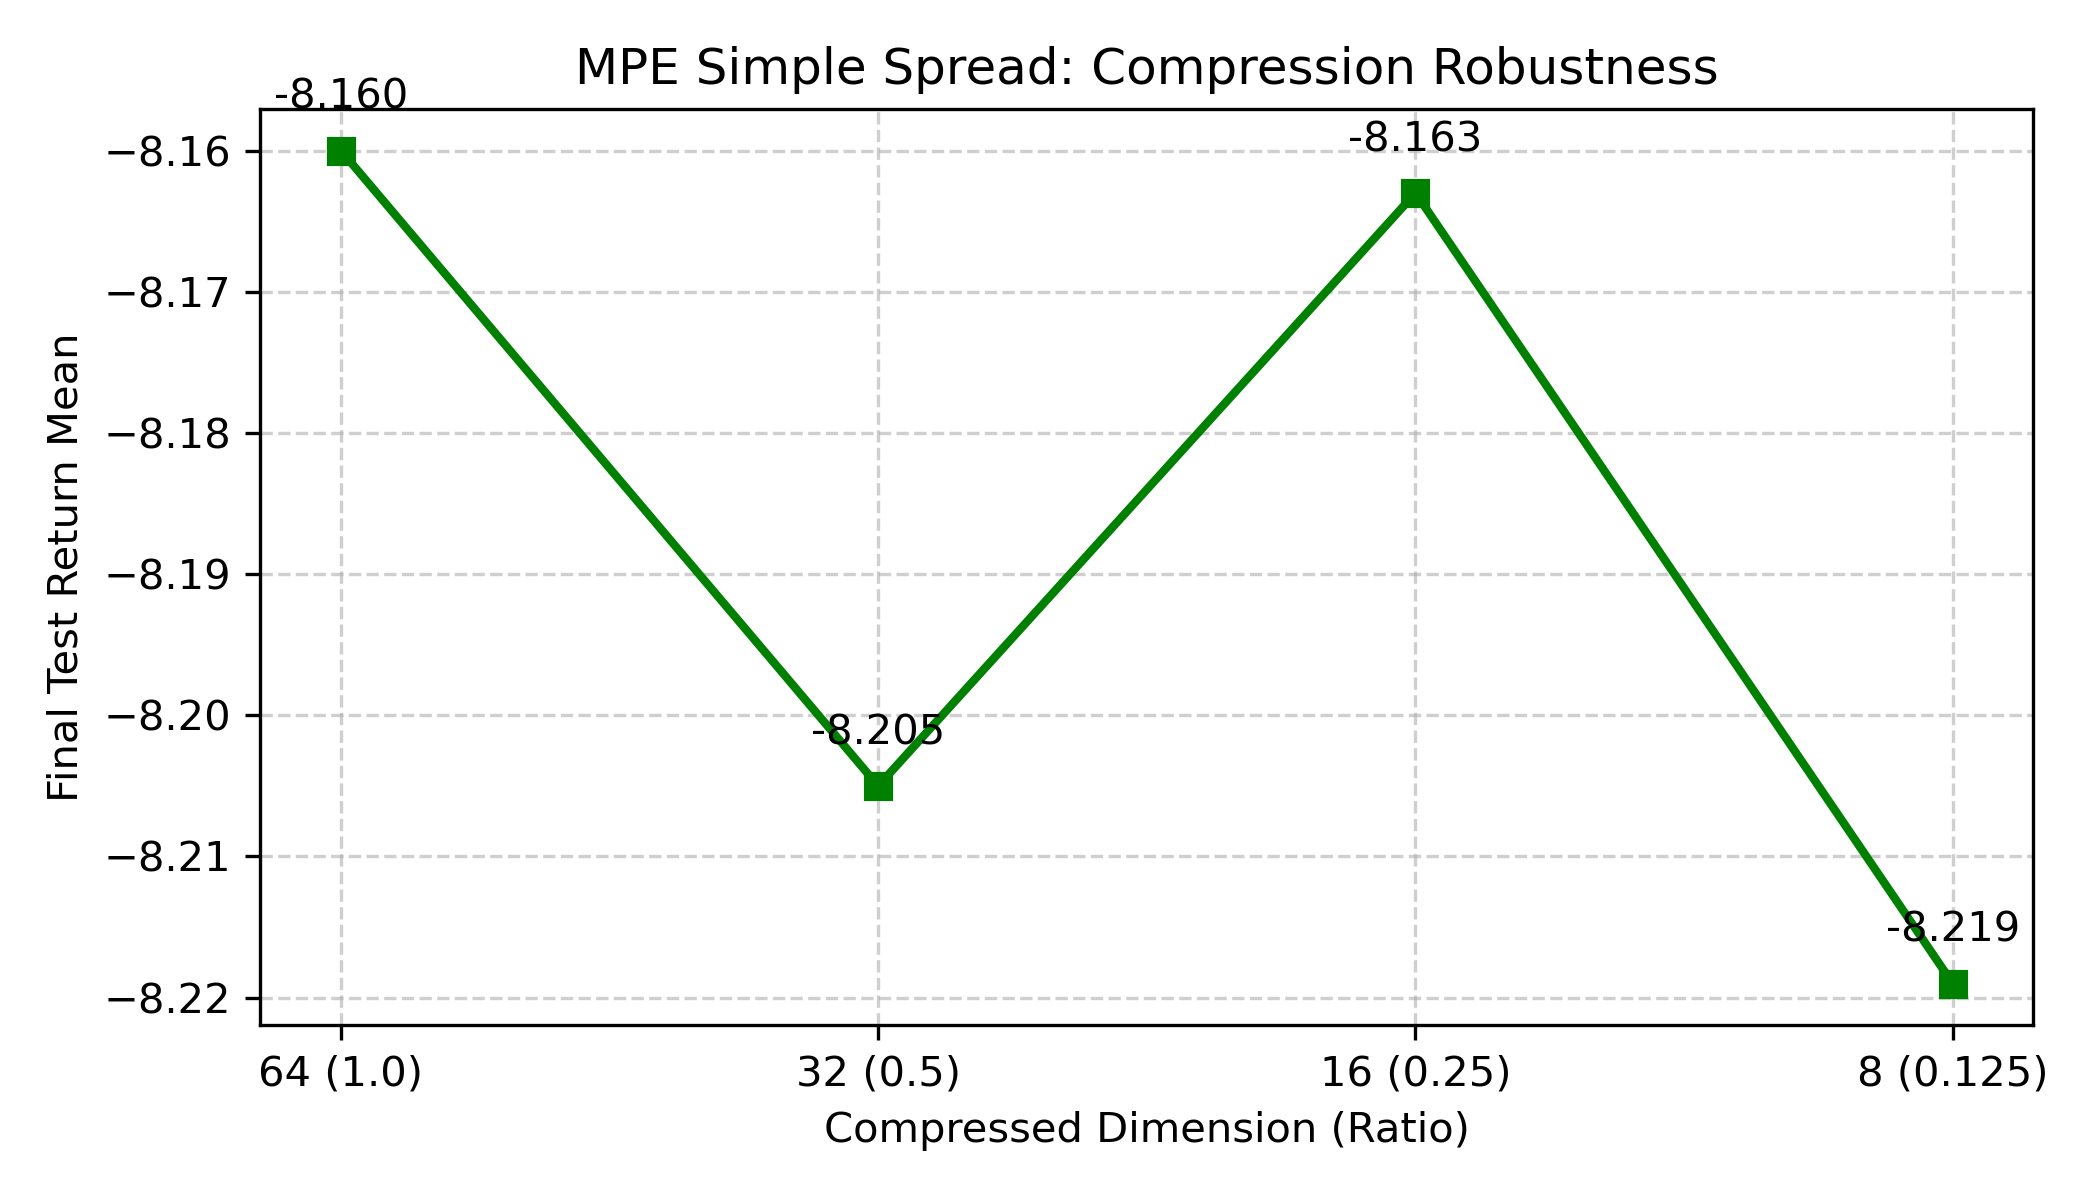
\includegraphics[width=\textwidth]{mpe_cr_ablation.png}
\caption{Compression ratio ablation.}
\label{fig:mpe_cr}
\end{minipage}
\end{figure}

\paragraph{Ablation: Compression Ratio.} We tested varying the compressed message dimension relative to the original hidden dimension (64). Figure~\ref{fig:mpe_cr} shows that compressing the message to a dimension of 8 (a 0.125$\times$ ratio) yields identical performance ($-$8.22) to the uncompressed dimension ($-$8.16). This confirms that ExpoComm-B achieves massive bandwidth savings without sacrificing performance.

%═══════════════════════════════════════════════════════════════════════════════
\section{Discussion and Limitations}
\label{sec:discussion}

\paragraph{Why does the bottleneck help?}
ExpoComm-B with moderate compression ($\sigma_0 = 0.01$) outperforms both uncompressed ExpoComm and QMIX despite less training. We hypothesize the variational bottleneck acts as a regularizer---forcing agents to extract and transmit only task-relevant information, similar to how dropout prevents overfitting. The auxiliary state-prediction loss provides a complementary learning signal that further grounds the compressed representations.

\textbf{Limitations.}
\textbf{(1)~Single seed:} All experiments used seed~123. Multi-seed runs (3--5 seeds) are required for statistical significance.
\textbf{(2)~Incomplete training (MAgent):} No run on MAgent completed the full 5.05M steps due to the 24-hour SLURM limit. QMIX reached 98\% while ExpoComm-B $\sigma_0{=}0.01$ reached only 66\%, making direct comparison imperfect.
\textbf{(3)~Non-monotonic ablation:} The result at $\sigma_0 = 0.02$ (worse than 0.01) on MAgent may reflect training incompleteness rather than a true property of the method.

\paragraph{Future work.}
Extending experiments to SMACv2, conducting multi-seed evaluations, scalability analysis across agent counts ($N = 5, 10, 20$), and investigating zero-shot generalization from small to large teams.

%═══════════════════════════════════════════════════════════════════════════════

\begin{ack}
We thank Prof.\ Arlei Silva for guidance throughout this project in COMP 559: Machine Learning with Graphs at Rice University. Computational resources were provided by the Rice University NOTS HPC cluster (Center for Research Computing). Experiment tracking was supported by Weights~\&~Biases. The ExpoComm-B codebase builds upon the open-source ExpoComm repository by Li et al.\ (Apache 2.0 license).
\end{ack}

%═══════════════════════════════════════════════════════════════════════════════
\section{Conclusion}
\label{sec:conclusion}

We introduced ExpoComm-B, a multi-agent communication architecture that jointly optimizes sparse communication topology and message bandwidth through the integration of ExpoComm's exponential graph structure with BVME's variational message compression. On the MAgent Battle benchmark with 81 cooperative agents, our best variant ($\sigma_0 = 0.05$) eliminates 95.6\% of opponent agents, compared to only 10.6\% for the no-communication QMIX baseline. On the MPE Simple Spread task, ExpoComm-B demonstrates robust superiority over both topology-only and compression-only baselines. The bandwidth ablation study reveals that $\sigma_0$ provides interpretable, monotonic control over the information--performance trade-off, while compression ratio ablations show we can reduce message sizes by $8\times$ without performance loss. Our work demonstrates that both \textit{who} to communicate with and \textit{how much} to communicate are essential dimensions that must be jointly optimized in bandwidth-constrained multi-agent systems.

\smallskip
\noindent\textbf{Code:}
\href{https://github.com/vt20-crypto/ExpoComm-B}{github.com/vt20-crypto/ExpoComm-B}
\quad
\textbf{W\&B:}
\href{https://wandb.ai/vt20-rice-university/ExpoComm-B}{wandb.ai/vt20-rice-university/ExpoComm-B}

%═══════════════════════════════════════════════════════════════════════════════
\bibliographystyle{unsrt}

\begin{thebibliography}{8}

\bibitem{expocomm}
X.~Li, X.~Wang, C.~Bai, J.~Zhang.
Exponential topology-enabled scalable communication in multi-agent reinforcement learning.
In \textit{ICLR}, 2025.

\bibitem{bvme}
W.~Duan, J.~Lu, E.~Yu, J.~Xuan.
Bandwidth-constrained variational message encoding for cooperative multi-agent reinforcement learning.
In \textit{AAMAS}, 2026.

\bibitem{tgcnet}
Z.~Zhang, B.~He, B.~Cheng, G.~Li.
Bridging training and execution via dynamic directed graph-based communication in cooperative multi-agent systems.
In \textit{AAAI}, 2025.

\bibitem{dgmappo}
S.~Shaik, J.~Smereka, Y.~Wang.
Multi-agent deep reinforcement learning under constrained communications.
\textit{arXiv:2601.17069}, 2026.

\bibitem{factored}
A.~Rashwan, K.~Briggs, C.~Budd, L.~Kreusser.
Factored value functions for graph-based multi-agent reinforcement learning.
\textit{arXiv:2601.11401}, 2026.

\bibitem{mfc}
T.~Schmidt, K.~Cui.
Mean-field control on sparse graphs.
\textit{arXiv:2601.21477}, 2026.

\bibitem{rlgsurvey}
M.~Nie, D.~Chen, D.~Wang.
Reinforcement learning on graphs: A survey.
\textit{IEEE TETCI}, 2023.

\bibitem{gnnmarl}
Z.~Liu et al.
Graph neural network meets multi-agent reinforcement learning: Fundamentals, applications, and future directions.
\textit{arXiv:2404.04898}, 2024.

\end{thebibliography}

\end{document}
